\subsection{p-Orbits}
\begin{figure}[h!]
\centering
\begin{subfigure}{0.48\textwidth}
    \centering
    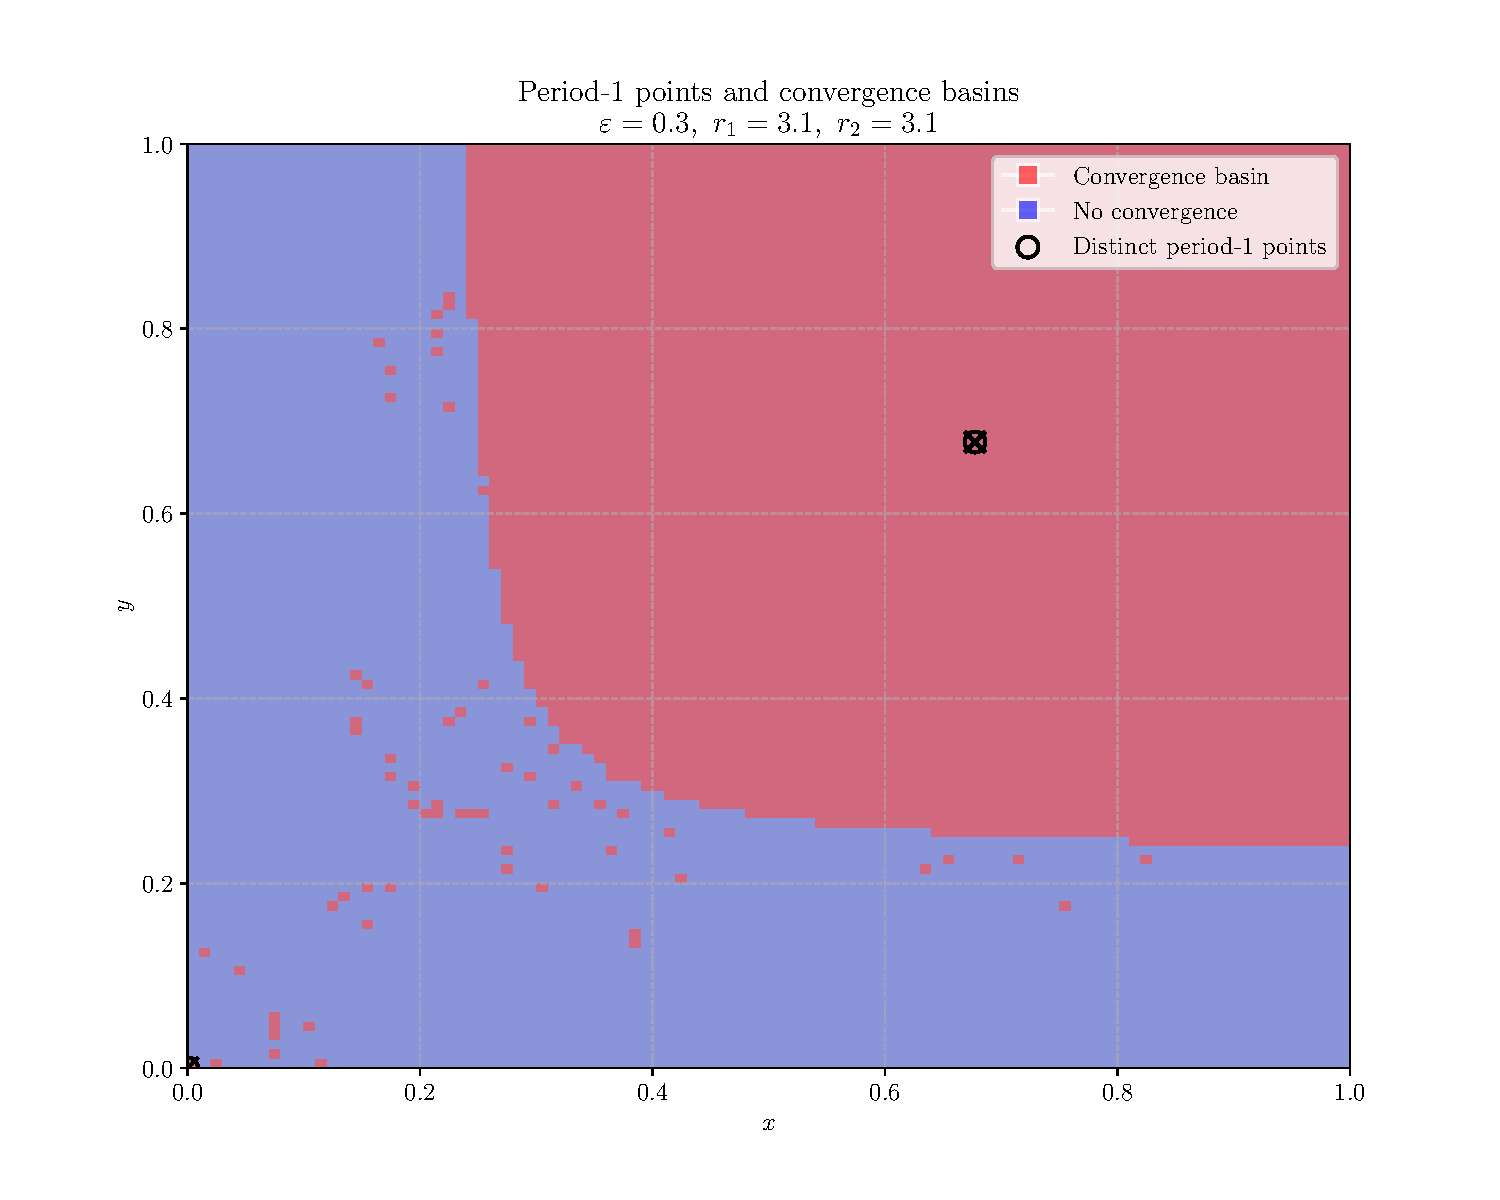
\includegraphics[width=\linewidth]{figs/1_0.3_3.1_3.1.pdf}
\end{subfigure}
\hfill
\begin{subfigure}{0.48\textwidth}
    \centering
    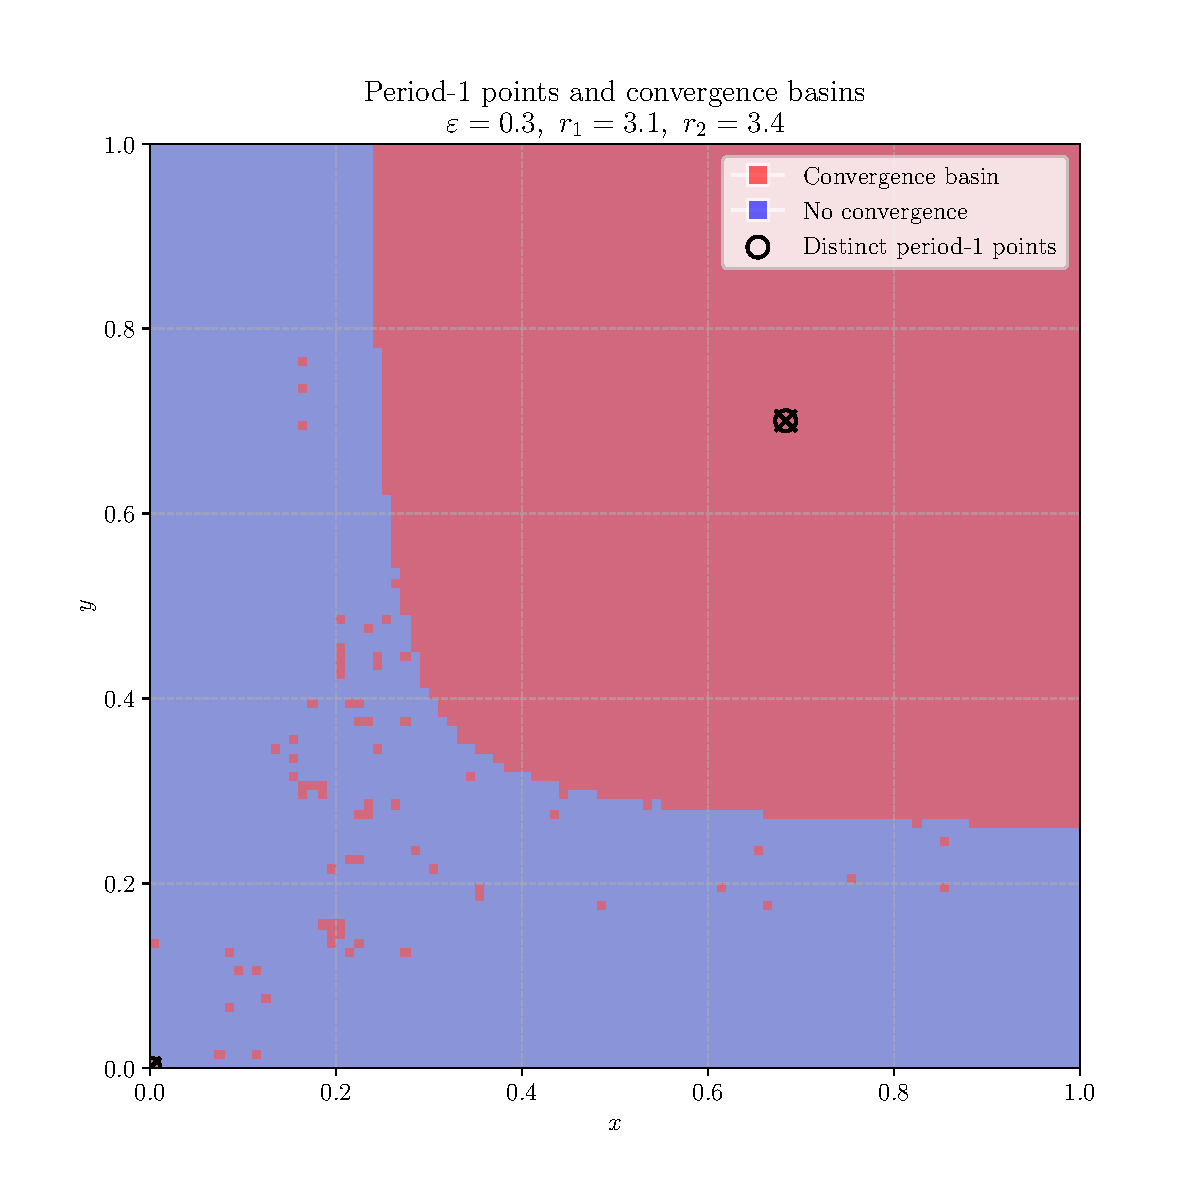
\includegraphics[width=\linewidth]{figs/1_0.3_3.1_3.4.pdf}
\end{subfigure}

\begin{subfigure}{0.48\textwidth}
    \centering
    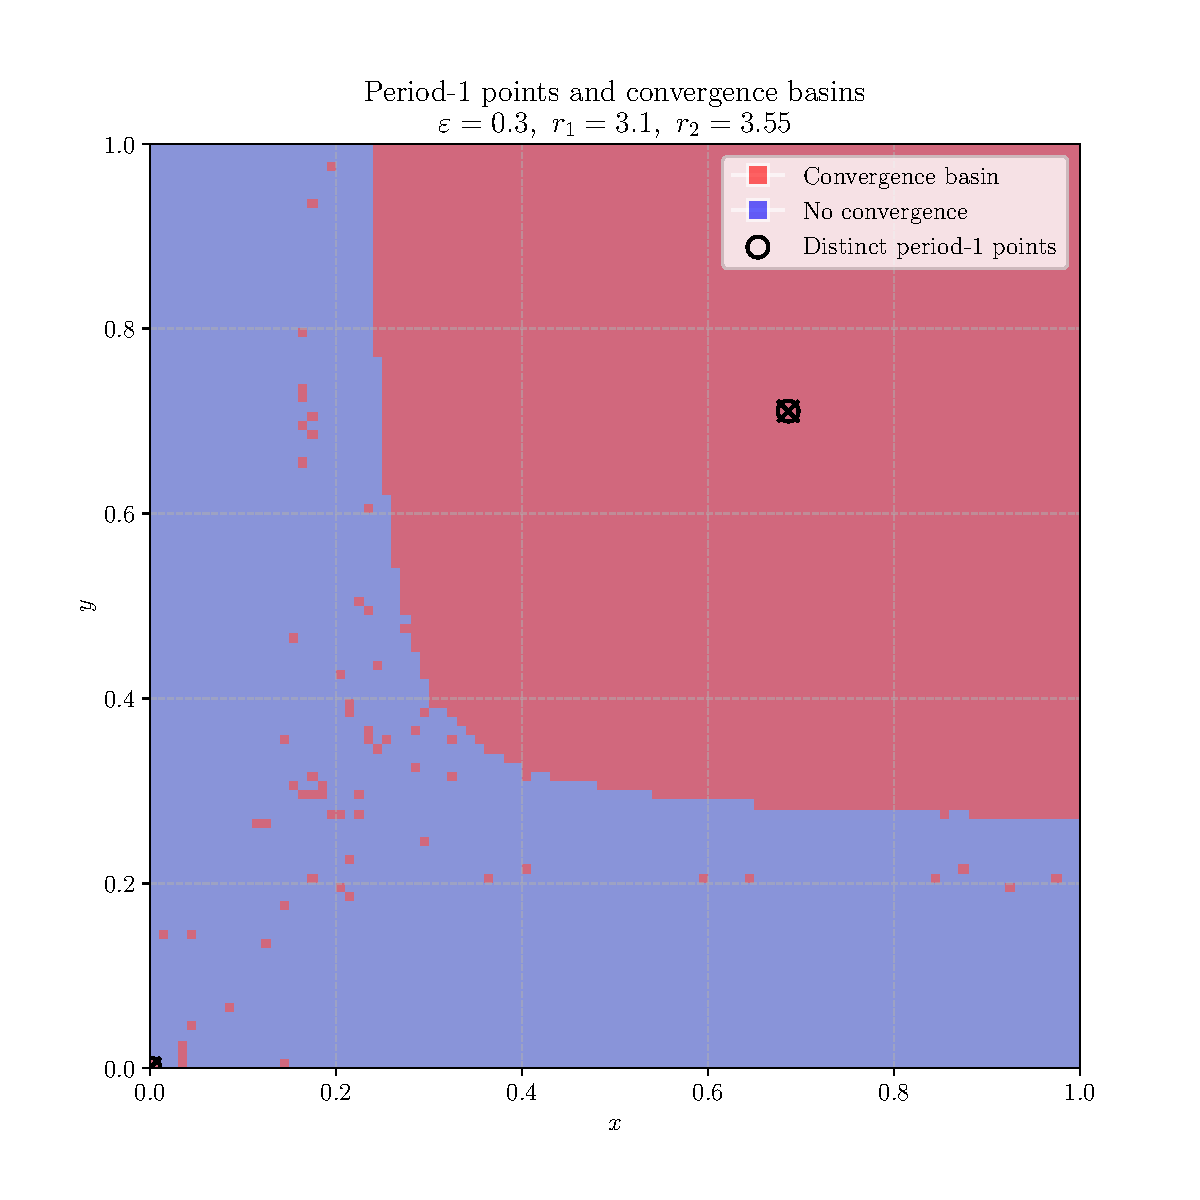
\includegraphics[width=\linewidth]{figs/1_0.3_3.1_3.55.pdf}
\end{subfigure}
\hfill
\begin{subfigure}{0.48\textwidth}
    \centering
    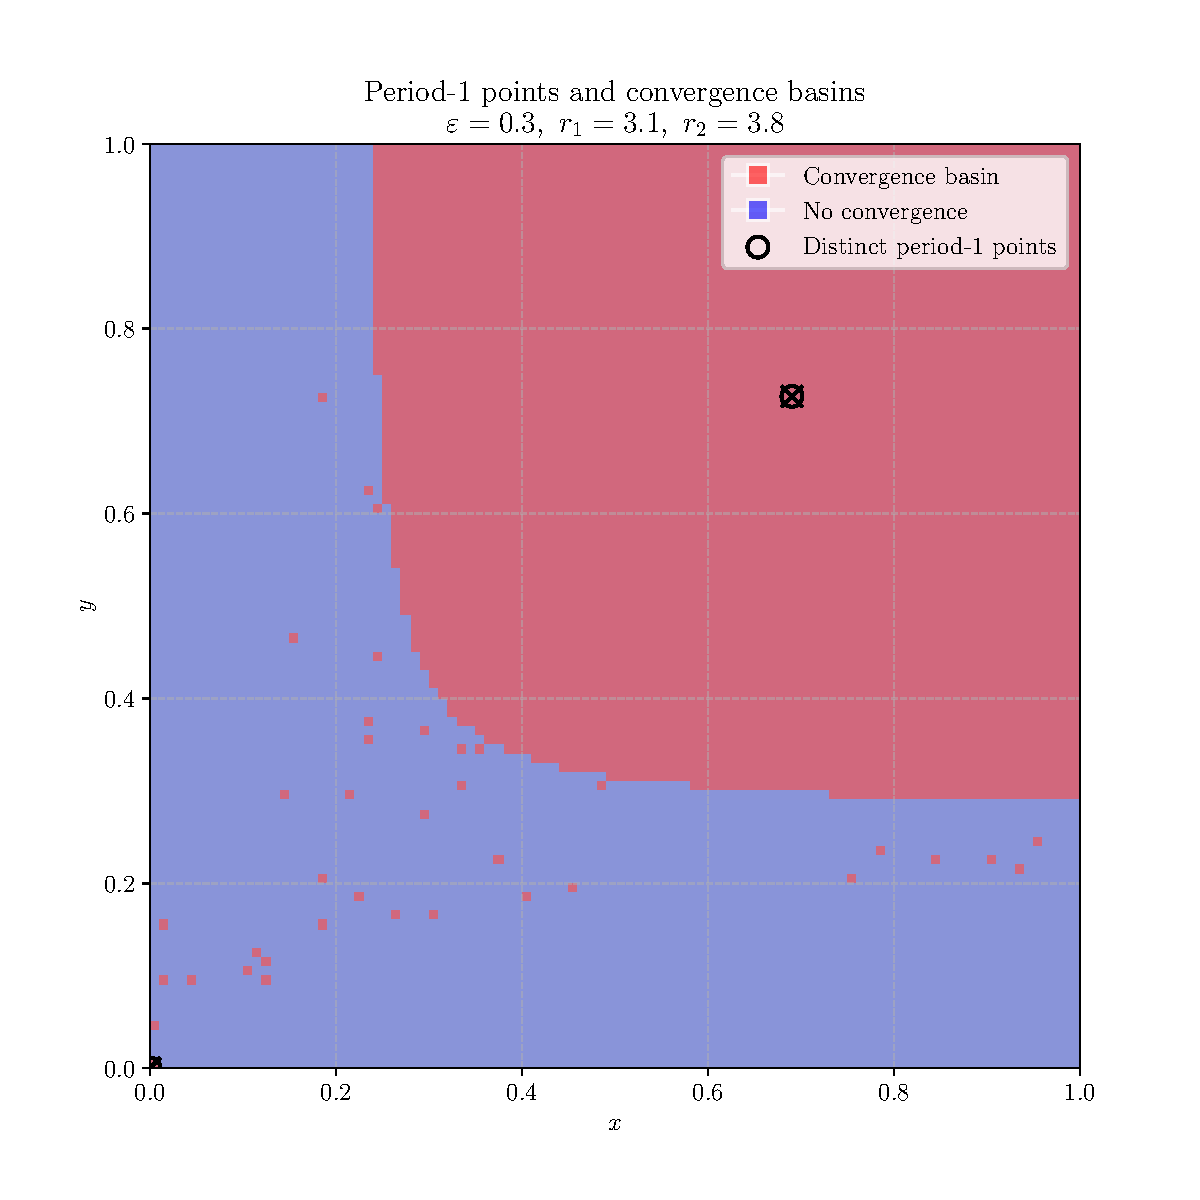
\includegraphics[width=\linewidth]{figs/1_0.3_3.1_3.8.pdf}
\end{subfigure}

\begin{subfigure}{0.48\textwidth}
    \centering
    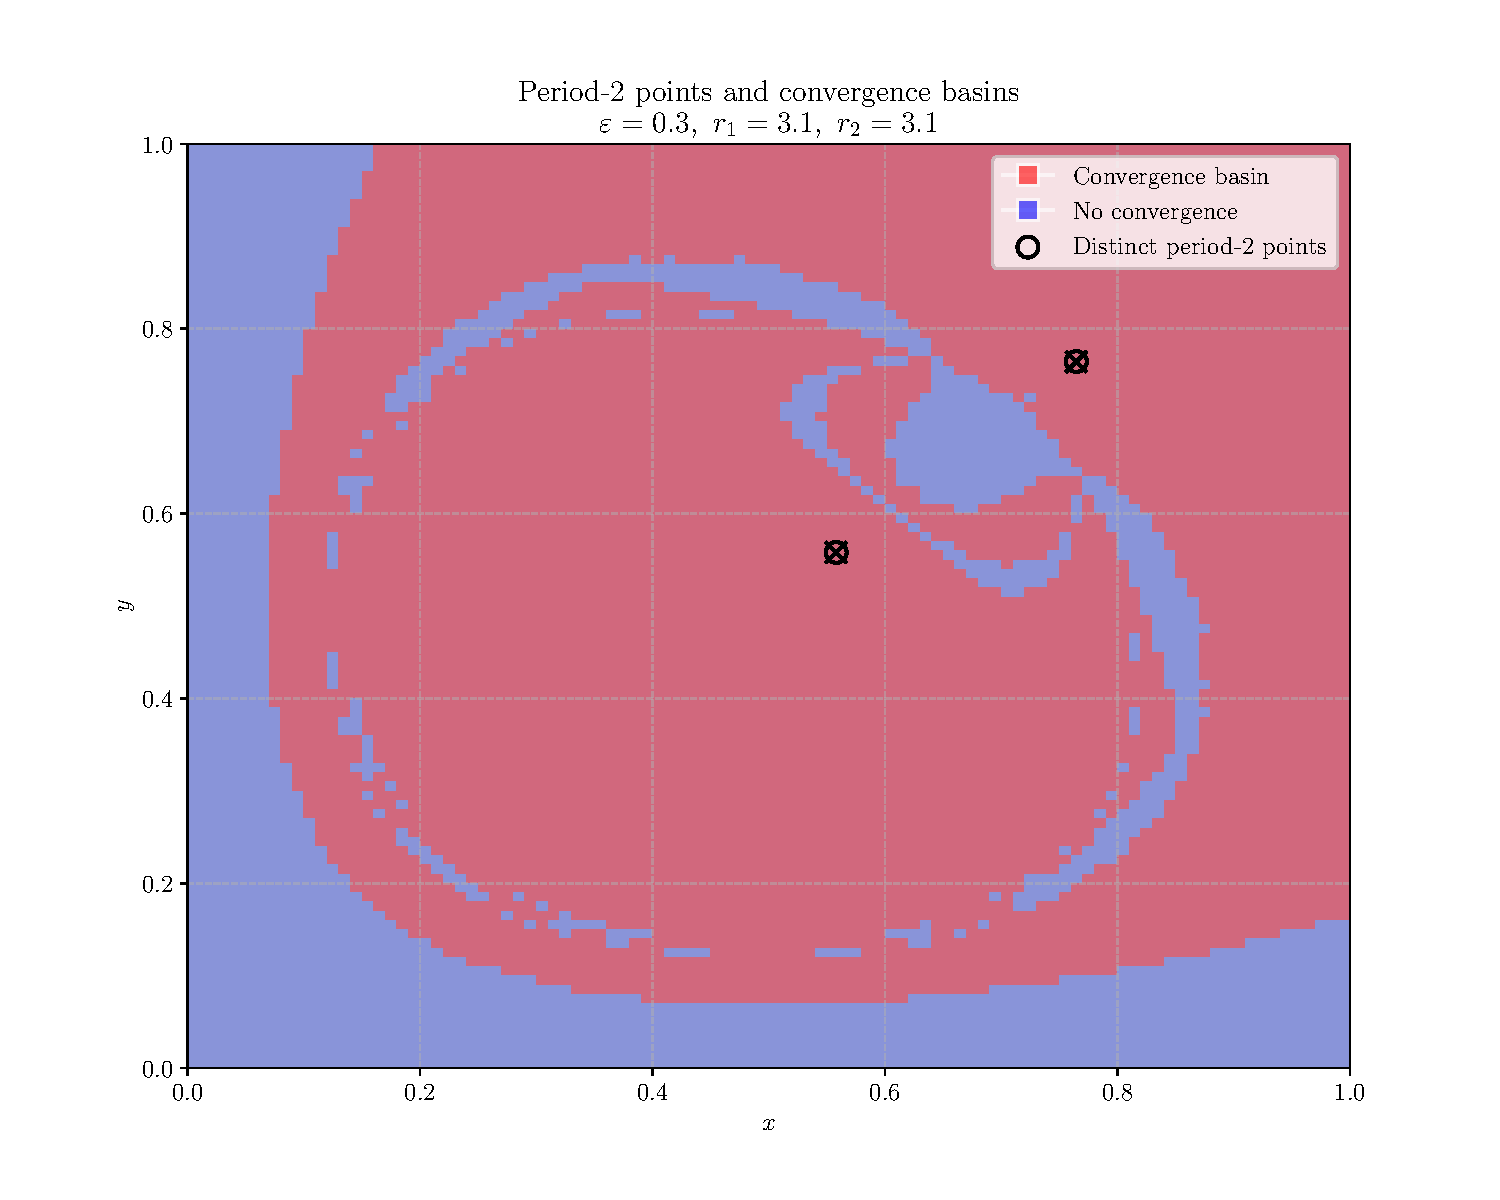
\includegraphics[width=\linewidth]{figs/2_0.3_3.1_3.1.pdf}
\end{subfigure}
\hfill
\begin{subfigure}{0.48\textwidth}
    \centering
    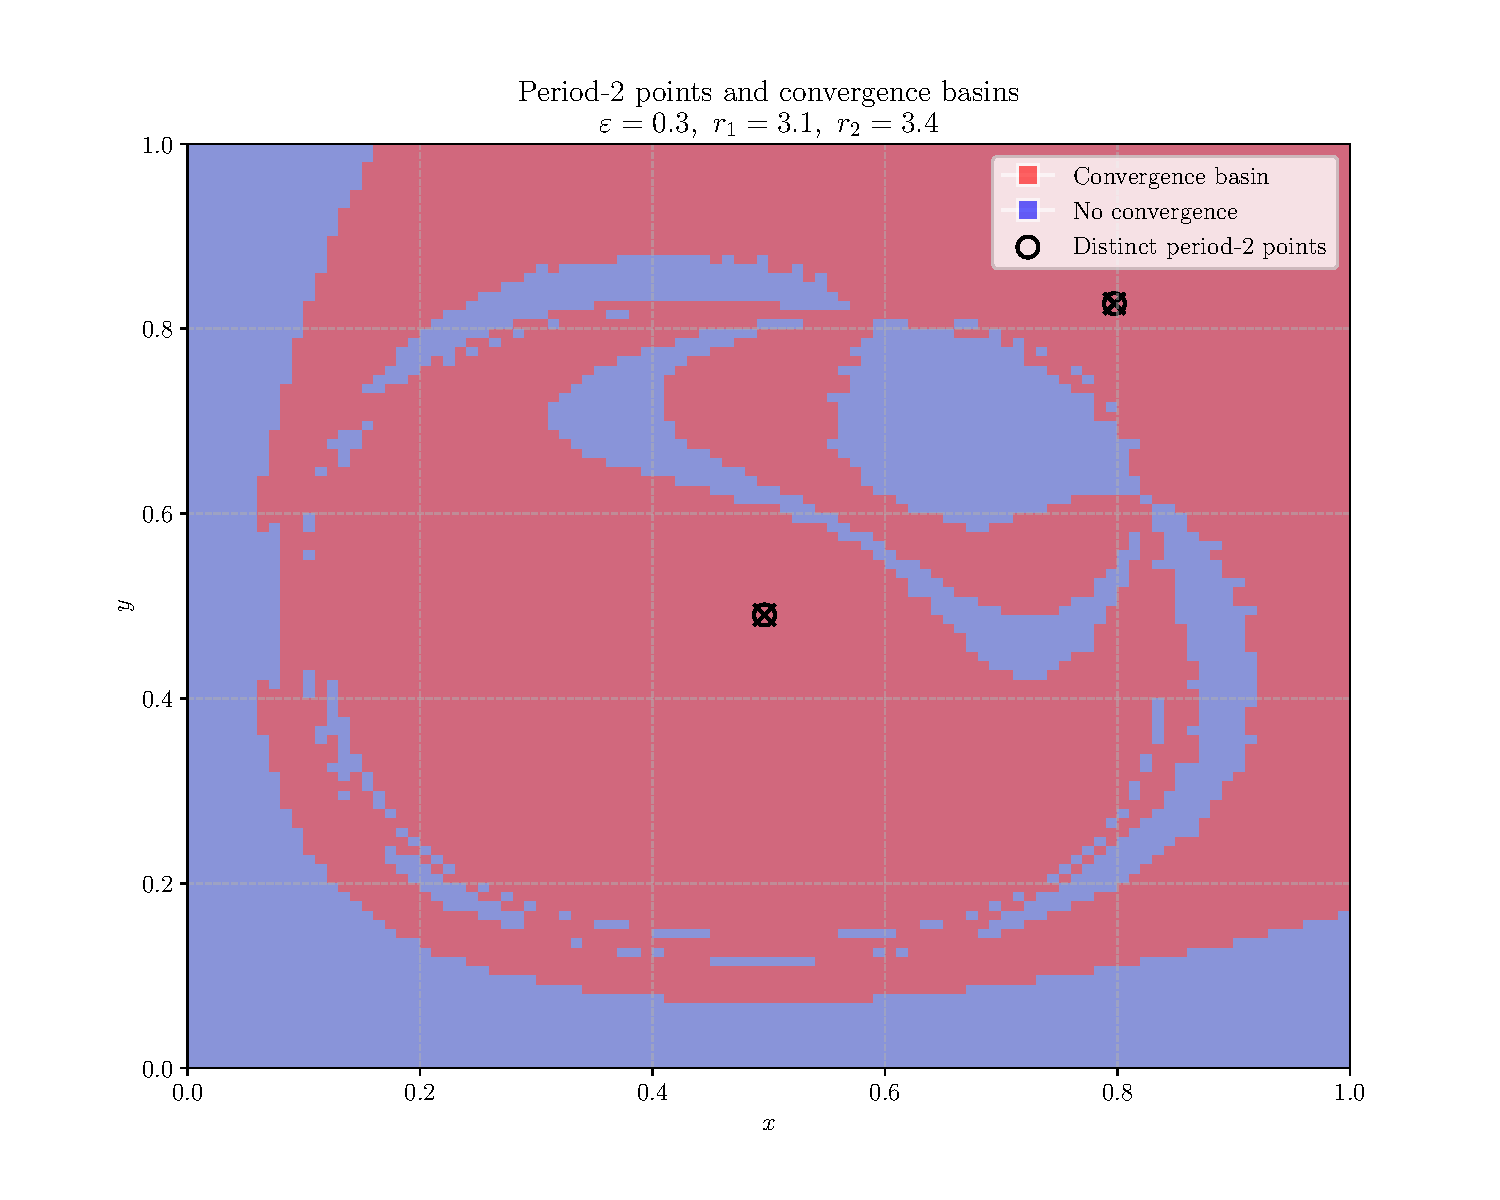
\includegraphics[width=\linewidth]{figs/2_0.3_3.1_3.4.pdf}
\end{subfigure}

\begin{subfigure}{0.48\textwidth}
    \centering
    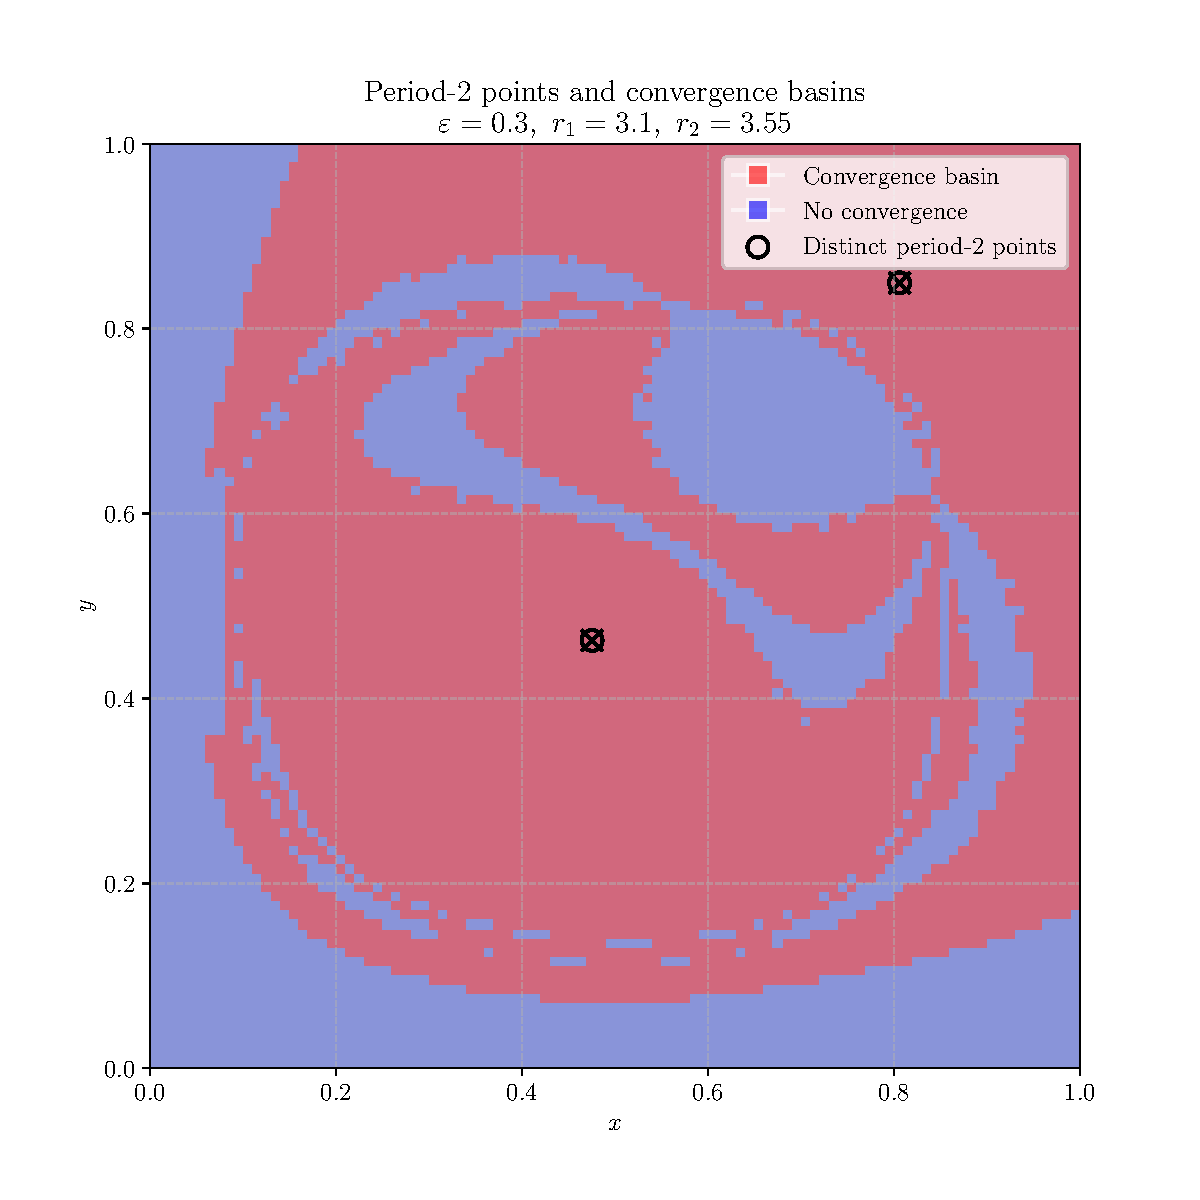
\includegraphics[width=\linewidth]{figs/2_0.3_3.1_3.55.pdf}
\end{subfigure}
\hfill
\begin{subfigure}{0.48\textwidth}
    \centering
    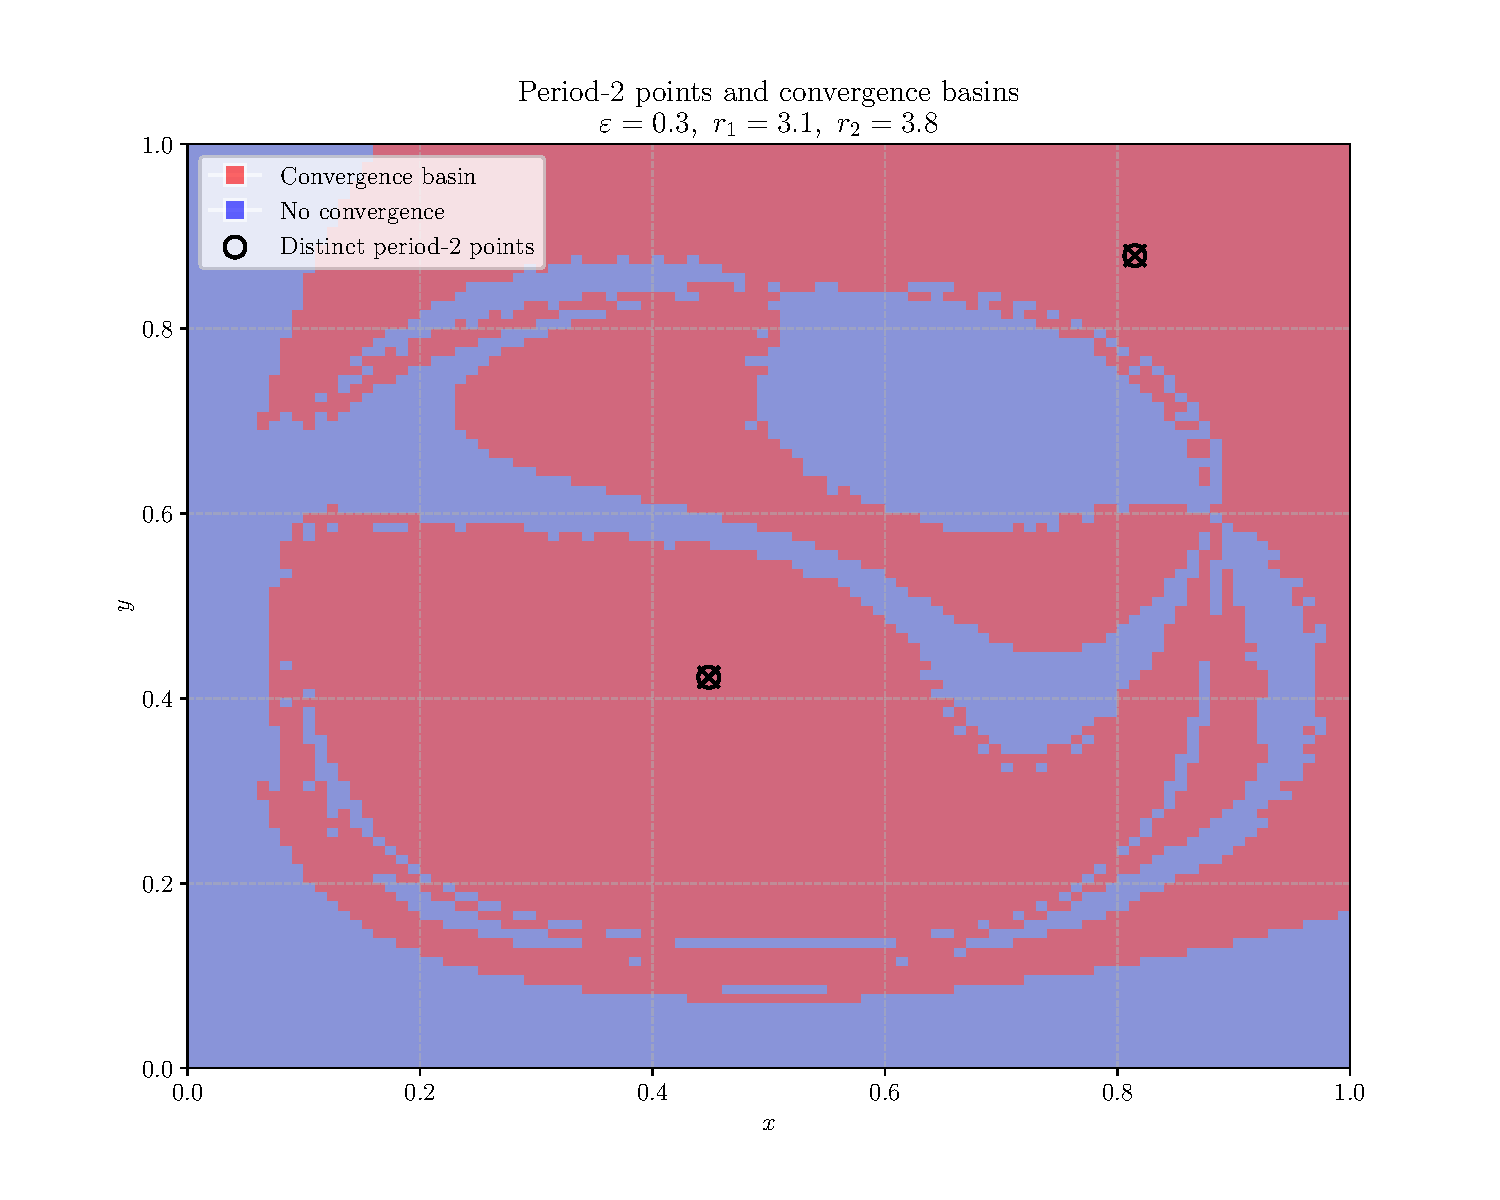
\includegraphics[width=\linewidth]{figs/2_0.3_3.1_3.8.pdf}
\end{subfigure}

\caption{4×2 subplot layout}
\label{fig:4x2}
\end{figure}
